\subsection{QuizziPedia::Back-End::App::Models}
\subsubsection{Informazioni generali}
\label{QuizziPedia::Back-End::App::Models}
\begin{figure}[ht]
	\centering
	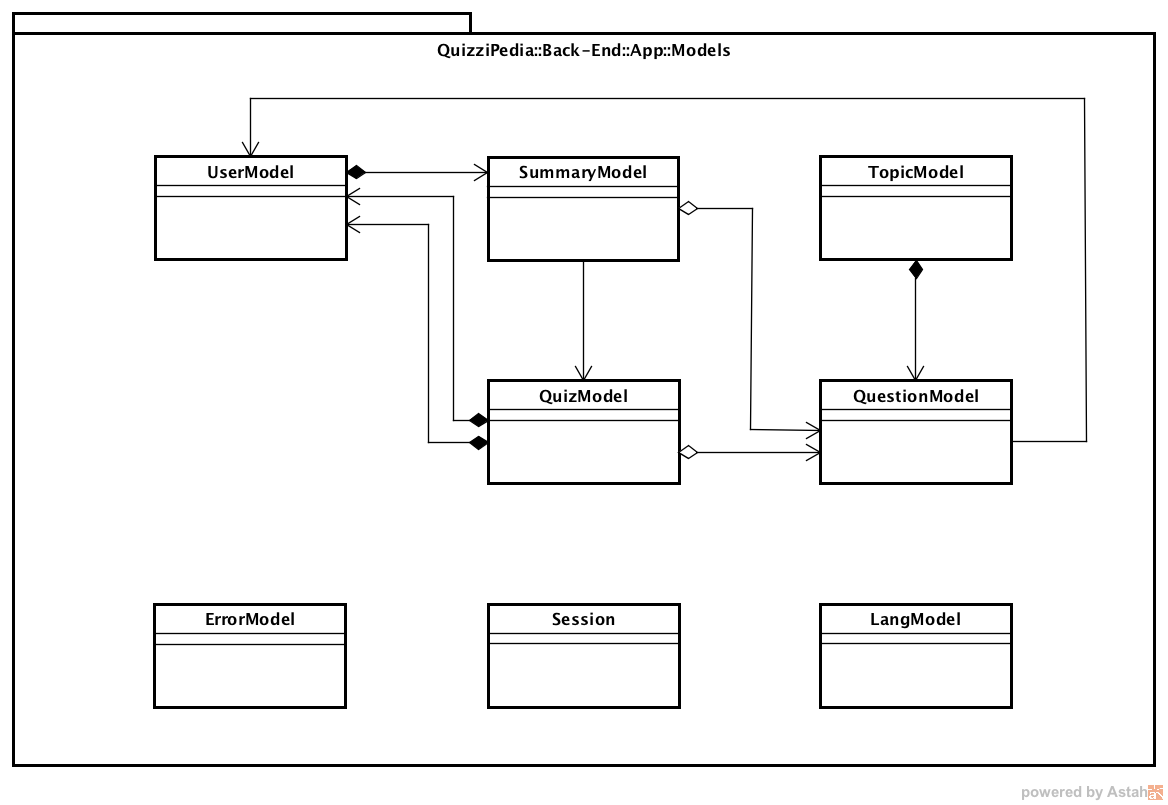
\includegraphics[scale=0.45]{UML/Package/QuizziPedia_Back-End_App_Models.png}
	\caption{QuizziPedia::Back-End::App::Models}
\end{figure}
\FloatBarrier
\begin{itemize}
	\item \textbf{Descrizione} \\
	\textit{Package\ped{G}} contenente le classi che definiscono il \textit{model} dell'applicazione. Queste classi sono definite come classi schema di \textit{Mongoose\ped{G}}, il quale permette di utilizzare \textit{MongoDB\ped{G}} tramite oggetti;
	\item \textbf{Padre} \texttt{App}
\end{itemize}

\subsubsection{Classi}
\paragraph{QuizziPedia::Back-End::App::Models::Session}
\label{QuizziPedia::Back-End::App::Models::Session}
\begin{figure}[ht]
	\centering
	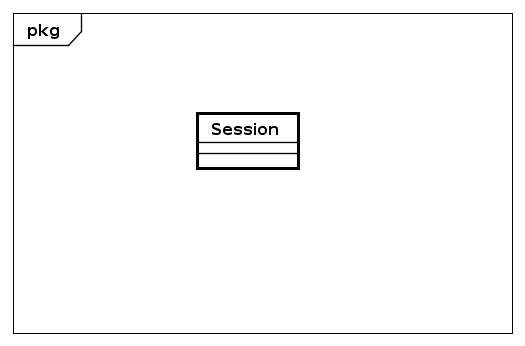
\includegraphics[scale=0.45]{UML/Classi/Back-End/QuizziPedia_Back-End_App_Models_sessionModel.png}
	\caption{QuizziPedia::Back-End::App::Models::Session}
\end{figure}
\FloatBarrier
	\begin{itemize}
		\item \textbf{Descrizione} \\
		Classe che gestisce la sessione utente dell'applicazione. Non sono stati modellati attributi e metodi di questa classe in quanto viene inizializzata da \textit{Express\ped{G}} ed utilizzata da \textit{Passport\ped{G}} attraverso funzionalità interne ai due \textit{middleware\ped{G}};
		\item \textbf{Utilizzo} \\
		Viene utilizzata da \textit{Passport\ped{G}} per memorizzare i dati della sessione che viene creata quando un utente effettua il login;
		\item \textbf{Relazioni con altre classi} \\
			\begin{itemize}
				\item
				IN \texttt{AuthenticationController} \\
				Classe che si occupa della registrazione e dell'autenticazione dell'utente nel sistema. È un componente ConcreteHandler del design pattern \textit{Chain of responsibility\ped{G}}. Risulta essere il componente che eventualmente esegue la richiesta del client attraverso \textit{Passport\ped{G}};			
				\item
				IN \texttt{SessionController} \\
				Classe \textit{middleware\ped{G}} che, utilizzando \textit{Passport\ped{G}}, si occupa di controllare la consistenza dell'oggetto session durante la sessione associata all'utente autenticato. È un componente ConcreteHandler del design pattern \textit{Chain of responsibility\ped{G}}.
			\end{itemize}
	\end{itemize}
\paragraph{QuizziPedia::Back-End::App::Models::UserModel}
\label{QuizziPedia::Back-End::App::Models::UserModel}
\begin{figure}
	\centering
	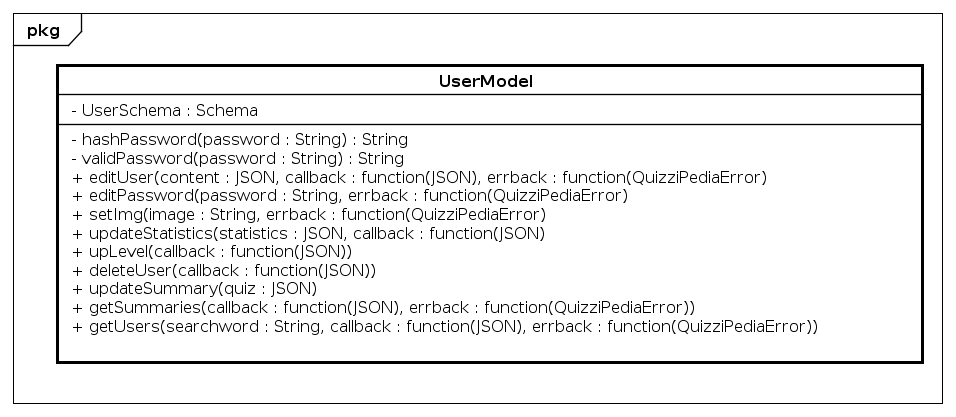
\includegraphics[scale=0.45]{UML/Package/QuizziPedia_Back-End_App_Models_userModel.png}
	\caption{QuizziPedia::Back-End::App::Models::UserModel}
\end{figure}
\begin{itemize}
	\item \textbf{Descrizione} \\
	Classe che modella la creazione e la gestione dei dati utente
	\item \textbf{Utilizzo} \\
	Viene utilizzata per rappresentare i dati degli account dei vari utenti dell'applicazione. Si interfaccia alla libreria Mongoose per la creazione dello schema e dei relativi metodi statici o di istanza.
	\item \textbf{Relazioni con altre classi} 
		\begin{itemize}
			\item \textbf{IN SummaryModel} \\
			Questa classe rappresenta il riepologo dei questionari svolti dagli utenti.
			\item \textbf{OUT QuestionModel} \\
			Questa classe rappresenta i dati delle domande create dai vari utenti.
			\item \textbf{OUT QuizModel} \\
			Questa classe rappresenta i dati dei questionari creati dagli utenti Pro.
			\item \textbf{OUT UserProModel} \\
			Questa classe rappresenta i dati riguardanti l'utente pro.
		\end{itemize}
	\item \textbf{Attributi} 
		\begin{itemize}
			\item \textbf{- \texttt{userSchema}: \texttt{Schema}} \\
			Questo campo dati rappresenta lo schema Mongoose dell'utente QuizziPedia. Lo schema prevede i seguenti attributi:
			\begin{itemize}
				\item 
					\texttt{name} di tipo \texttt{String}, rappresenta il nome  dell'utente registrato;
				\item 
					\texttt{surname} di tipo \texttt{String}, rappresenta il cognome  dell'utente registrato;
				\item 
					\texttt{email} di tipo \texttt{String}, rappresenta l'email  dell'utente registrato;
				\item 
					\texttt{userImg} di tipo \texttt{String}, rappresenta il path della foto profilo dell'utente registrato;
				\item 
					\texttt{username} di tipo \texttt{String}, rappresenta l'username con cui viene identificato l'utente all'interno dell'applicazione;		
				\item
					\texttt{password} di tipo \texttt{String}, rappresenta la password associata all'utente,  appositamente codificata mediante l'algoritmo bcrypt;  		
				\item
					\texttt{statistics} di tipo \texttt{Array Mixed}, contenente i seguenti attributi:
				\begin{itemize}
					\item
						\texttt{topicName} di tipo \texttt{String}, rappresenta il nome della statistica relativa all'argomento;	 
					\item
						 \texttt{topicLevel} di tipo \texttt{Number}, identifica il livello di preparazione dell'utente in un determinato argomento;
					\item
						\texttt{correctAnswers} di tipo \texttt{Number}, identifica il numero di risposte corrette date dall'utente riguardanti domande di un determinato argomento; 
					\item						
						 \texttt{totalAnswers} di tipo \texttt{Number} , identifica il numero di risposte totali date dall'utente riguardanti domande di un determinato argomento.		
				\end{itemize}		
				\item 
					\texttt{levelUsers} di tipo \texttt{Number}, identifica il livello dell'utente;				
				
				\item
					\texttt{quizSummaries} di tipo \texttt{Array}, contiene oggetti di tipo \texttt{ObjectId}, che rappresentano i riferimenti agli identificativi nel database dei questionari svolti dall'utente;		
			\end{itemize}	
		\end{itemize}	
	\item \textbf{Metodi}
		\begin{itemize}
		\item
		- \texttt{hashPassword(password: String): String} \\
		Effettua l'hashing della stringa password se non è già stata criptata tramite campo salt per evitare attacchi di tipo rainbow. \\
		\textbf{Parametri} 
			\begin{itemize}
			\item
				 \texttt{password: String} \\
				Rappresenta la password dell'utente.
			\end{itemize}
		\item
		- \texttt{validPassword(password: String): String} \\
		Effettua la validità della password inserita comparandola con la password criptata.	\\
		\textbf{Parametri} 
			\begin{itemize}
			\item
				\texttt{password: String} \\
				Rappresenta la password inserita dall'utente.
			\end{itemize}
		\item
		+ \texttt{editUser(content: JSON, callback: function(JSON), errback: function(QuizzipediaError))} \\
		Questo metodo aggiorna i dati personali dell'utente. Restituisce un oggetto JSON che descrive l’elemento dopo l’aggiornamento oppure un messaggio di errore.	\\
		\textbf{Parametri} 
			\begin{itemize}
			\item
				\texttt{content: JSON} \\
				Rappresenta i dati dell'utente da aggiornare.
			\item	
				\texttt{callback: function(JSON)} \\
				Rappresenta la callback che il metodo deve chiamare al termine dell'elaborazione.
			\item	
				\texttt{errback: function(QuizzipediaError)} \\
				Questo parametro rappresenta la callback che il metodo deve chiamare qualora si verificassero errori nell'esecuzione del metodo.
			\end{itemize}	
		+ \texttt{editPassword(password: String, errback: function(QuizzipediaError))} \\
		Questo metodo aggiorna la password vecchia dell'utente con quella passata per parametro. Restituisce un messaggio di errore nel caso in cui si verificati dei problemi nel cambio della password.	\\
		\textbf{Parametri} 
			\begin{itemize}
			\item
				\texttt{password: String} \\
				Rappresenta la nuova password dell'utente da sostituire a quella vecchia.
			\item	
				\texttt{errback: function(QuizzipediaError)} \\
				Questo parametro rappresenta la callback che il metodo deve chiamare qualora si verificassero errori nell'esecuzione del metodo.
			\end{itemize}
		+ \texttt{setImg(image : String, errback : function(QuizziPediaError))} \\	
		Questo metodo aggiorna l'immagine profilo dell'utente. Restituisce un messaggio di errore nel caso in cui si verificati dei problemi nell'aggiornamento dell'immagine.	\\	
		\textbf{Parametri} 
			\begin{itemize}
			\item
				\texttt{image: String} \\
				Rappresenta l'immagine per aggiornare la foto del profilo.
			\item	
				\texttt{errback: function(QuizzipediaError)} \\
				Questo parametro rappresenta la callback che il metodo deve chiamare qualora si verificassero errori nell'esecuzione del metodo.
			\end{itemize}
		+ \texttt{updateStatistics(statistics : JSON, callback : function(JSON))} \\	
		Questo metodo aggiorna le statistiche dell'utente in un determinato argomento. Restituisce un oggetto JSON che descrive le statistiche dell'utente dopo l'aggiornamento.	\\	
		\textbf{Parametri} 
			\begin{itemize}
			\item
				\texttt{statistics: JSON} \\
				Rappresenta il contenuto delle statistiche riguardanti l'esercitazione effettuata in un determinato argomento da utilizzare per aggiornare quelle esistenti .
			\item	
				\texttt{callback: function(JSON)} \\
				Rappresenta la callback che il metodo deve chiamare al termine dell'elaborazione.
			\end{itemize}	
		+ \texttt{upLevel(callback : function(JSON))} \\
		Questo metodo aggiorna il livello di difficoltà relativo alla capacità dell'utente a rispondere a determinate domande. Restituisce un oggetto JSON che descrive il livello dell'utente dopo l'aggiornamento.	\\	
		\textbf{Parametri} 
			\begin{itemize}
			\item	
				\texttt{callback: function(JSON)} \\
				Rappresenta la callback che il metodo deve chiamare al termine dell'elaborazione.		
			\end{itemize}	
		+ \texttt{deleteUser(callback : function(JSON), errback:function(QuizzipediaError))} \\	
		Questo metodo elimina dal sistema l'utente registrato. Restituisce un oggetto JSON che descrive i dati dell'utente eliminato.	\\	
		\textbf{Parametri} 
			\begin{itemize}
			\item	
				\texttt{callback: function(JSON)} \\
				Rappresenta la callback che il metodo deve chiamare al termine dell'elaborazione.	
			\item	
				\texttt{errback: function(QuizzipediaError)} \\
				Questo parametro rappresenta la callback che il metodo deve chiamare qualora si verificassero errori nell'esecuzione del metodo.		
			\end{itemize}
		+ \texttt{updateSummary(quiz : JSON)}	
		Questo metodo aggiorna la cronologia dell'utente in relazione ai questionari svolti.\\	
		\textbf{Parametri} 
			\begin{itemize}
			\item	
				\texttt{quiz : JSON)} \\
				Rappresenta il contenuto del questionario svolto .		
			\end{itemize}
		+ \texttt{getSummaries(callback : function(JSON), errback : function(QuizziPediaError))}	
		Questo metodo ritorna un JSON contenente la cronologia dei questionari svolti da parte dell'utente, in caso di errori una callback che segnalerà i relativi problemi.\\
		\textbf{Parametri} 
			\begin{itemize}
			\item	
				\texttt{callback: function(JSON)} \\
				Rappresenta la callback che il metodo deve chiamare al termine dell'elaborazione.	
			\item	
				\texttt{errback: function(QuizzipediaError)} \\
				Questo parametro rappresenta la callback che il metodo deve chiamare qualora si verificassero errori nell'esecuzione del metodo.	
		+ \texttt{getUsers(searchword : String, callback : function(JSON), errback : function(QuizziPediaError))}		
		Questo metodo ritorna un JSON contenente i dati degli utenti in base alla parola chiave cercata, in caso di errori una callback che segnalerà i relativi problemi.\\
		\textbf{Parametri} 
			\begin{itemize}
			\item	
				\texttt{searchword: String} \\
				Rappresenta la parola chiave cercata in base alla quale verrà filtrata la ricerca degli utenti.	
			\item	
				\texttt{callback: function(JSON)} \\
				Rappresenta la callback che il metodo deve chiamare al termine dell'elaborazione.	
			\item	
				\texttt{errback: function(QuizzipediaError)} \\
				Questo parametro rappresenta la callback che il metodo deve chiamare qualora si verificassero errori nell'esecuzione del metodo.		
			\end{itemize}
		\end{itemize}	
\end{itemize}
\paragraph{QuizziPedia::Back-End::App::Models::UserProModel}
\label{QuizziPedia::Back-End::App::Models::UserProModel}
\begin{figure}
	\centering
	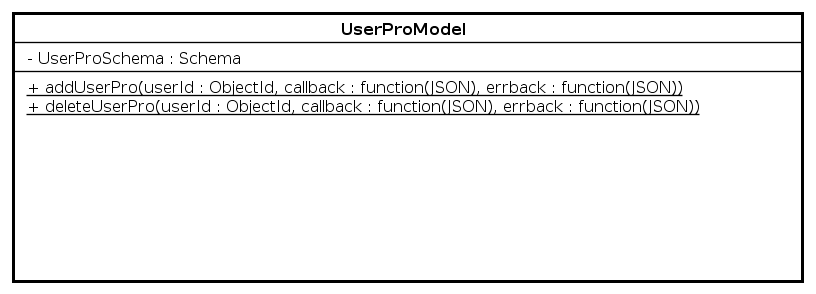
\includegraphics[scale=0.45]{UML/Classi/Back-End/QuizziPedia_Back-End_App_Models_userProModel.png}
	\caption{QuizziPedia::Back-End::App::Models::UserProModel}
\end{figure}
\FloatBarrier
\begin{itemize}
	\item \textbf{Descrizione} \\
	Classe che modella i dati dell'utente pro.
	\item \textbf{Utilizzo} \\
	Viene utilizzata per rappresentare i dati dell'utente pro. Si interfaccia alla libreria Mongoose per la creazione dello schema e dei relativi metodi statici o di istanza.
	\item \textbf{Relazioni con altre classi} 
		\begin{itemize}
			\item IN \textbf {UserManagementController} \\
			Classe che gestisce la logica applicativa riguardante la visualizzazione e la modifica dei dati dell'utente.
Rappresenta il ConcreteHandler nel design pattern Chain of responsibility. Utilizza Passport.
			\item IN \textbf{QuizModel} \\
			Questa classe rappresenta i dati dei questionari creati dagli utenti Pro.
			\item OUT \textbf{UserModel} \\
			Questa classe rappresenta i dati riguardanti i vari utenti registrati al sistema.
		\end{itemize}
	\item \textbf{Attributi} 
		\begin{itemize}
			\item \textbf{- \texttt{UserProSchema}: \texttt{Schema}} \\
			Questo campo dati rappresenta lo schema Mongoose dell'utente pro QuizziPedia. Lo schema prevede i seguenti attributi:
			\begin{itemize}
				\item 
					\texttt{userID} di tipo \texttt{ObjectId}, rappresenta il riferimento all'identificativo nel database contenente i dati dei vari utenti registrati;
			\end{itemize}		
		\end{itemize}	
	\item \textbf{Metodi}
		\begin{itemize}
		\item
		+ \texttt{addUserPro(userId : ObjectId, callback: function(JSON), errback: function(QuizzipediaError))} \\	
		Questo metodo è statico ed aggiorna la tipologia di utenza. In specifico l'utente di tipo basic passerà a pro. Ritorna un JSON contenente i dati del nuovo utente pro, qualora si siano verificati problemi verrà ritornato un messaggio d'errore.	\\	
		\textbf{Parametri} 
			\begin{itemize}
			\item
				\texttt{userId: ObjectId} \\
				Rappresenta l'identificativo dell'utente da passare a pro
			\item	
				\texttt{callback: function(JSON)} \\
				Rappresenta la callback che il metodo deve chiamare al termine dell'elaborazione.	
			\item	
				\texttt{errback: function(QuizzipediaError)} \\
				Questo parametro rappresenta la callback che il metodo deve chiamare qualora si verificassero errori nell'esecuzione del metodo.		
			\end{itemize}	
		\item	
		+ \texttt{deleteUserPro(userId : ObjectId, callback: function(JSON), errback: function(QuizzipediaError))} \\	
		Questo metodo è statico ed aggiorna la tipologia di utenza. In specifico l'utente di tipo pro ritornerà a basic, eliminando il riferimento alla classe user . Ritorna un JSON contenente i dati dell'utente pro ritornato a basic, qualora si siano verificati problemi verrà ritornato un messaggio d'errore.	\\	
		\textbf{Parametri} 
			\begin{itemize}
			\item
				\texttt{userId: ObjectId} \\
				Rappresenta l'identificativo dell'utente pro da ritornare a basic
			\item	
				\texttt{callback: function(JSON)} \\
				Rappresenta la callback che il metodo deve chiamare al termine dell'elaborazione.	
			\item	
				\texttt{errback: function(QuizzipediaError)} \\
				Questo parametro rappresenta la callback che il metodo deve chiamare qualora si verificassero errori nell'esecuzione del metodo.		
			\end{itemize}		
		\end{itemize}
		
\end{itemize}
\paragraph{QuizziPedia::Back-End::App::Models::QuestionModel}
\label{QuizziPedia::Back-End::App::Models::QuestionModel}
\begin{figure}[ht]
	\centering
	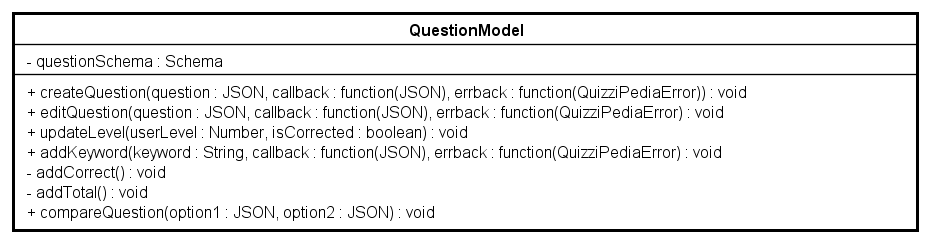
\includegraphics[scale=0.45]{UML/Classi/Back-End/QuizziPedia_Back-End_App_Models_questionModel.png}
	\caption{QuizziPedia::Back-End::App::Models::QuestionModel}
\end{figure}
\FloatBarrier
	\begin{itemize}
		\item \textbf{Descrizione} \\
		Classe che modella i dati relativi alle domande all'interno dell'applicazione;	
		\item \textbf{Utilizzo} \\
		Viene utilizzata per rappresentare le domande. Si interfaccia alla libreria \textit{Mongoose\ped{G}} per la creazione dello schema e dei relativi metodi statici o di istanza;
		\item \textbf{Relazione con altra classi}:
			\begin{itemize}
			\item IN \textbf{UserModel} \\
			Classe che rappresenta tutti gli utenti;
			\item OUT \textbf{SummaryModel} \\
			Classe che rappresenta i riepiloghi dei questionari svolti;
			\item OUT \textbf{TopicModel} \\
			Classe che rappresenta gli argomenti;
			\item OUT \textbf{QuizModel} \\
			Classe che modella i questionari all'interno dell'applicazione;
			\end{itemize}
		\item \textbf{Attributi}:
	\begin{itemize}
		\item \texttt{questionSchema: Schema} \\
		Questo campo dati rappresenta lo schema Mongoose per le domande e prevede i seguenti attributi:
		\begin{itemize}
			\item \texttt{author} di tipo \texttt{ObjectId}, rappresenta il riferimento all'identificativo nel database dell'utente che ha creato la domanda;
			\item \texttt{type} di tipo \texttt{String}, rappresenta la tipologia di domanda;
			\item \texttt{language} di tipo \texttt{String}, rappresenta la lingua in cui è scritta la domanda; 
			\item \texttt{questionText} di tipo \texttt{String}, rappresenta il testo della domanda; 
			\item \texttt{image} di tipo \texttt{String}, rappresenta l'URL dell'immagine associata al testo della domanda;
			\item \texttt{options1} di tipo \texttt{Array}, contiene oggetti di tipo String e rappresenta informazioni diverse in base alla tipologia della domanda;
			\item \texttt{options2} di tipo \texttt{Array}, contiene oggetti di tipo String e rappresenta informazioni diverse in base alla tipologia della domanda;
			\item \texttt{level} di tipo \texttt{Number}, rappresenta la difficoltà della domanda;
			\item \texttt{totalAnswers} di tipo \texttt{Number}, rappresenta le risposte totali che tutti gli utenti hanno dato alla domanda;
			\item \texttt{correctAnswers} di tipo \texttt{Number}, rappresenta quante risposte corrette hanno dato gli utenti che hanno risposto alla domanda.
		\end{itemize}
	\end{itemize}
\item \textbf{Metodi}:
	\begin{itemize}
	\item \texttt{+ createQuestion(question: JSON, callback: function(JSON),\\ errback: function(QuizziPediaError))} \\
	Metodo che permette la creazione di una nuova domanda; \\
		\textbf{Parametri}:
		\begin{itemize}
			\item \texttt{question: JSON} \\
			Rappresenta le informazioni che andranno a comporre la domanda da creare;
			\item \texttt{callback: function(JSON)} \\
			Rappresenta la \textit{callback\ped{G}} che verrà eseguita al termine dell'elaborazione nel caso non si verifichino errori durante l'esecuzione;
			\item \texttt{errback: function(QuizziPediaError)} \\
			Rappresenta la \textit{callback\ped{G}} che il metodo deve chiamare qualora si verificassero errori durante l'esecuzione del metodo.
		\end{itemize}   
	\item \texttt{+ editQuestion(question: JSON, callback: function(JSON),\\ errback: function(QuizziPediaError))} \\
	Metodo che permette di modificare una domanda già esistente; \\
		\textbf{Parametri}:
		\begin{itemize}
			\item \texttt{question : JSON} \\
			Rappresenta le nuove informazioni che andranno a modificare le informazioni precedenti di una specifica domanda;
			\item \texttt{callback: function(JSON)} \\
			Rappresenta la \textit{callback\ped{G}} che verrà eseguita al termine dell'elaborazione del metodo in caso non si verifichino errori durante l'esecuzione;
			\item \texttt{errback: function(QuizziPediaError)} \\
			Rappresenta la \textit{callback\ped{G}} che il metodo deve chiamare qualora si verificassero errori durante l'esecuzione del metodo.
		\end{itemize}
	\item \texttt{+ addKeyword(keyword: String, callback: function(JSON),\\ errback: function(QuizziPediaError))} \\
	Metodo che permette di aggiungere delle parole chiave ad una specifica domanda; \\
		\textbf{Parametri}:
			 \begin{itemize}
			 	\item \texttt{keyword: String} \\
			 	Rappresenta la parola chiave da inserire
			 	\item \texttt{callback: function(JSON)} \\
			 	Rappresenta la \textit{callback\ped{G}} che verrà eseguita al termine dell'elaborazione del metodo in caso si verifichino errori durante l'esecuzione;
			 	\item \texttt{errback: function(QuizziPediaError)} \\
			 	Rappresenta la \textit{callback\ped{G}} che il metodo deve chiamare qualora si verificassero errori durante l'esecuzione del metodo.
			 \end{itemize}
	\item \texttt{+ updateLevel(userLevel: Number, isCorrected: boolean)} \\
	Metodo che permette di aggiornare il livello di difficoltà della domanda, questo metodo è chiamato ogni qualvolta un utente risponde ad una domanda durante un allenamento;
		\textbf{Parametri}:
			\begin{itemize}
				\item \texttt{userLevel: Number} \\
				Indica, con un numero compreso tra 1 e 1000, l'abilità dell'utente che ha risposto alla domanda;
				\item \texttt{isCorrected: boolean} \\
				Indica se l'utente che ha risposto alla domanda ha risposto correttamente.
			\end{itemize}  
	\item \texttt{- addCorrect()} \\
	Metodo che permette di incrementare il contatore di risposte corrette di una determinata domanda;
	\item \texttt{- addTotal()} \\
	Metodo che permette di incrementare il contatore delle risposte date di una determinata domanda.
	\item \texttt{+ compareAnswers(option1: JSON, option2: JSON)}
	Metodo che serve per confrontare le risposte date dagli utenti con le risposte effettive delle domande per sapere se sono corrette, ogni tipologia di domanda tratterà in modo diverso i parametri per confrontare il proprio metodo di risposta; \\
	\textbf{Parametri:}
		\begin{itemize}
			\item \texttt{option1: JSON} \\
			Rappresenta la prima parte della risposta fornita dall'utente;
			\item \texttt{option2: JSON} \\
			Rappresenta la seconda parte della risposta fornita dall'utente;
		\end{itemize}
	\end{itemize}
\end{itemize}

\paragraph{QuizziPedia::Back-End::App::Models::QuizModel}
\label{QuizziPedia::Back-End::App::Models::QuizModel}
\begin{figure}
	\centering
	\includegraphics[scale=0.45]{UML/Package/QuizziPedia_Back-End_App_Models_QuizModel.png}
	\caption{QuizziPedia::Back-End::App::Models::QuizModel}
\end{figure}
\paragraph{QuizziPedia::Back-End::App::Models::TopicModel}
\label{QuizziPedia::Back-End::App::Models::TopicModel}
\begin{figure}
	\centering
	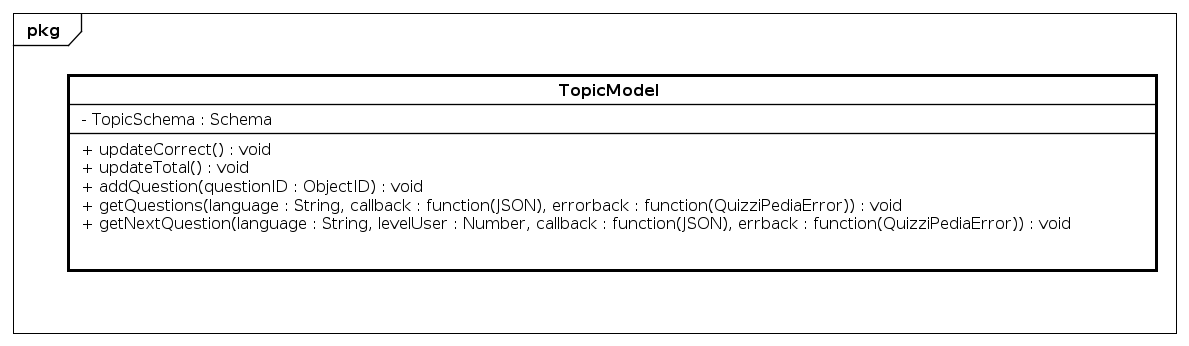
\includegraphics[scale=0.45]{UML/Classi/Back-End/QuizziPedia_Back-End_App_Models_topicModel.png}
	\caption{QuizziPedia::Back-End::App::Models::TopicModel}
\end{figure}
\begin{itemize}
	\item \textbf{Descrizione} \\
	Classe che modella gli argomenti all'interno delle domande.
	\item \textbf{Utilizzo} \\
	Viene utilizzata per rappresentare i dati relativi agli argomenti delle domande. Si interfaccia con la libreria \textit{Mongoose\ped{G}} per la creazione dello schema e dei relativi metodi statici o di istanza.
	\item \textbf{Relazioni con altre classi}
		\begin{itemize}
			\item \textbf{IN \texttt{QuestionModel}} \\
			Questa classe rappresenta i dati delle domande create dai vari utenti;
			\item \textbf{IN \texttt{UserModel}} \\
			Questa classe rappresenta gli utenti.
		\end{itemize}
	\item \textbf{Attributi}
		\begin{itemize}
			\item \textbf{- topicSchema: Schema} \\
			Questo campo dati rappresenta lo schema \textit{Mongoose\ped{G}} per gli argomenti e prevede i seguenti attributi:
				\begin{itemize}
					\item \texttt{name} di tipo \texttt{String}, rappresenta il nome dell'argomento;
					\item \texttt{correctAnswers} di tipo \texttt{Number}, rappresenta il numero totale di domande alle quali gli utenti hanno risposto correttamente durante un allenamento sull'argomento; 
					\item \texttt{totalAnswers} di tipo \texttt{Number}, rappresenta il numero totale di domande alle quali gli utenti hanno risposto durante un allenamento sull'argomento;
					\item \texttt{question} di tipo \texttt{Array}, contiene gli \texttt{ObjectId} delle domande sull'argomento.
				\end{itemize}
		\end{itemize}
	\item \textbf{Metodi}
		\begin{itemize}
			\item \texttt{+ updateCorrect() : void} \\
			Metodo che consente di tenere aggiornato il numero di risposte esatte date a domande sull'argomento.
			\item \texttt{+ updateTotal() : void} \\
			Metodo che consente di tenere aggiornato il numero totale di risposte date a domande sull'argomento.
			\item \texttt{+ addQuestion(questionID : ObjectID) : void} \\
			Metodo che consente di aggiunge una domanda tra le domande sull'argomento. \\
			\textbf{Parametri}:
			\begin{itemize}
			\item \texttt{questionId : ObjectId} \\
			Rappresenta l'identificativo della domanda da aggiungere.
			\end{itemize}
			\item \texttt{+ getQuestions(language : String, callback : function(JSON), errback : function(QuizziPediaError)) : void} \\
			Metodo che consente di ottenere le domande sull'argomento attraverso la funzione di callback oppure un messaggio di errore. \\
			\textbf{Parametri}:
			\begin{itemize}
			\item \texttt{language : String} \\
			Rappresenta la lingua in cui sono scritte le domande che si vuole ottenere;
			\item \texttt{callback : function(JSON)} \\
			Rappresenta la callback che il metodo deve chiamare al termine dell'elaborazione nel caso in cui non si siano verificati errori;
			\item \texttt{errback : function(QuizziPediaError)} \\
			Rappresenta la callback che il metodo deve chiamare qualora si verificassero errori durante l'esecuzione del metodo.
			\end{itemize}
			\item \texttt{+ getNextQuestion(language : String, levelUser : Number, callback : function(JSON), errback : function(QuizziPediaError)) : void} \\
			Metodo che consente di ottenere la domanda successiva nella modalità allenamento, in base al livello dell'utente che lo sta svolgendo. \\
			\textbf{Parametri}:
			\begin{itemize}
			\item \texttt{language : String} \\
			Rappresenta la lingua in cui è scritta la domanda che si vuole ottenere;
			\item \texttt{levelUser : Number} \\
			Rappresenta il livello dell'utente che sta svolgendo l'allenamento;
			\item \texttt{callback : function(JSON)} \\
			Rappresenta la callback che il metodo deve chiamare al termine dell'elaborazione nel caso in cui non si siano verificati errori;
			\item \texttt{errback : function(QuizziPediaError)} \\
			Rappresenta la callback che il metodo deve chiamare qualora si verificassero errori durante l'esecuzione del metodo.
			\end{itemize}
		\end{itemize}
\end{itemize}
\paragraph{QuizziPedia::Back-End::App::Models::SummaryModel}
\label{QuizziPedia::Back-End::App::Models::summaryModel}
\begin{figure}
	\centering
	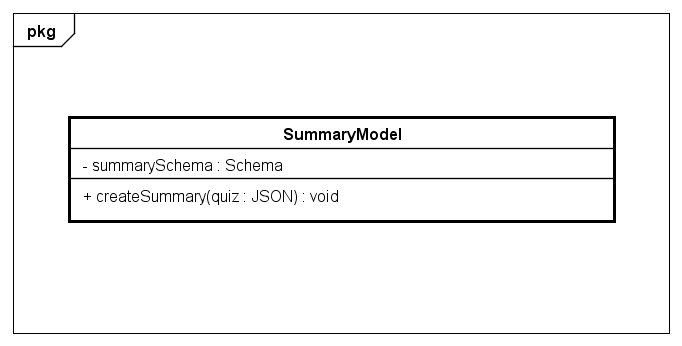
\includegraphics[scale=0.45]{UML/Package/QuizziPedia_Back-End_App_Models_summaryModel.png}
	\caption{QuizziPedia::Back-End::App::Models::summaryModel}
\end{figure}



\begin{itemize}
	\item \textbf{Descrizione} \\
	Classe che modella i riepiloghi all'interno dell'applicazione.
	\item \textbf{Utilizzo} \\
	Viene utilizzata per rappresentare i dati relativi ai riepiloghi all'interno dell'applicazione. Si interfaccia con la libreria \textit{Mongoose\ped{G}} per la creazione dello schema e dei relativi metodi statici o di istanza.
	\item \textbf{Relazioni con altre classi}
		............
	\item \textbf{Attributi}
		\begin{itemize}
			\item \textbf{- summarySchema: Schema} \\
			Questo campo dati rappresenta lo schema \textit{Mongoose\ped{G}} dei riepiloghi di \progetto. Lo schema prevede i seguenti attributi:
				\begin{itemize}
					\item \texttt{quiz} di tipo \texttt{ObjectId}, rappresenta il riferimento all'identificativo nel database del quiz;
					\item \texttt{givenAnswers} di tipo \texttt{Array}, contiene oggetti di tipo \texttt{ObjectId} che rappresentano i riferimenti agli identificativi nel database delle domande a cui si è risposto e due \texttt{Array} contenenti oggetti di tipo \texttt{String};	
					\item \texttt{date} di tipo \texttt{Date}, rappresenta la data di creazione del riepilogo.
				\end{itemize}
		\end{itemize}
	\item \textbf{Metodi}
		\begin{itemize}
			\item \texttt{+ createSummary(quiz: JSON)}\\
			Crea un riepilogo.\\
			\textbf{Parametri}:
			\begin{itemize}
				\item \texttt{quiz: JSON}\\
				Rappresenta il quiz dalle cui risposte verrà creato il riepilogo.
			\end{itemize}
		\end{itemize}
\end{itemize}
\paragraph{QuizziPedia::Back-End::App::Models::LangModel}
\label{QuizziPedia::Back-End::App::Models::LangModel}
\begin{figure}[ht]
	\centering
	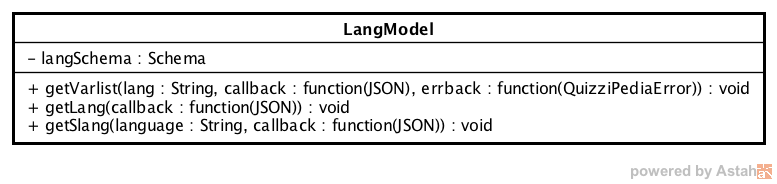
\includegraphics[scale=0.45]{UML/Classi/Back-End/QuizziPedia_Back-End_App_Models_langModel.png}
	\caption{QuizziPedia::Back-End::App::Models::LangModel}
\end{figure}
\FloatBarrier
	\begin{itemize}
		\item \textbf{Descrizione}: classe che modella le informazioni riguardanti la lingua dell'applicazione;
		\item \textbf{Utilizzo}: viene utilizzata per scambiare memorizzare le traduzioni delle variabili che andranno visualizzate nella \textit{view\ped{G}}.
		\item \textbf{Relazioni con altre classi}:
			\begin{itemize}
				\item OUT LangController \\
				Classe che gestisce la logica applicativa riguardante la traduzione delle variabili;
			\end{itemize}
		\item \textbf{Attributi}:
			\begin{itemize}
				\item \texttt{LangSchema : Schema} \\
				Questo campo rappresenta lo schema \textit{mongoose\ped{G}} per le variabili della lingua e prevede i seguenti attributi:
					\begin{itemize}
						\item \texttt{lang} di tipo \texttt{String}, rappresenta la lingua scelta per l'applicazione;
						\item \texttt{eng} di tipo \texttt{Array}, contiene oggetti con coppie di tipo \texttt{String} che associano i nomi delle variabili alla loro traduzione in inglese;
						\item \texttt{ita} di tipo \texttt{Array}, contiene oggetti con coppie di tipo \texttt{String} che associano i nomi delle variabili alla loro traduzione in italiano;
					\end{itemize}
			\end{itemize}
		\item \textbf{Metodi}:
			\begin{itemize}
				\item \texttt{+ getVarlist(lang: String, callback: function(JSON), \\ errback: function(QuizziPediaError))} \\
				Metodo che permette di ritornare la traduzione delle variabili; \\
				\textbf{Parametri}:
					\begin{itemize}
						\item \texttt{lang: String} \\
						Rappresenta l'informazione che indica il set di traduzione da ritornare;
						\item \texttt{callback: function(JSON)} \\
						Rappresenta la \textit{callback\ped{G}} che verrà eseguita al termine dell'elaborazione nel caso non si verifichino errori durante l'esecuzione;
						\item \texttt{errback: function(QuizziPediaError)} \\
						Rappresenta la \textit{callback\ped{G}} che verrà eseguito al termine dell'elaborazione nel caso si verifichino errori durante l'esecuzione del metodo;
					\end{itemize}
			\end{itemize}
	\end{itemize}
	
\paragraph{QuizziPedia::Back-End::App::Models::ErrorModel}
\label{QuizziPedia::Back-End::App::Models::ErrorModel}
\begin{figure}[ht]
	\centering
	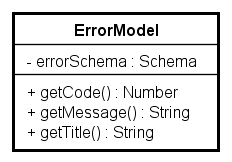
\includegraphics[scale=0.45]{UML/Classi/Back-End/QuizziPedia_Back-End_App_Models_errorModel.png}
	\caption{QuizziPedia::Back-End::App::Models::ErrorModel}
\end{figure}
\FloatBarrier
\begin{itemize}
	\item \textbf{Descrizione} \\
	Classe che rappresenta le informazioni di un errore che si è verificato eseguendo una determinata operazione.
	\item \textbf{Utilizzo} \\
	Viene utilizzata per racchiudere tutte le informazioni riguardanti l'errore.
	\item \textbf{Relazioni con altre classi}
		\begin{itemize}
			\item \textbf{IN \texttt{ErrorHandler}} \\
			Classe \textit{middleware\ped{G}} per la gestione degli errori. Ritorna al \textit{client\ped{G}} un oggetto di tipo \texttt{Response} con stato \textit{HTTP\ped{G}} 500 e descrizione dell'errore in formato \textit{JSON\ped{G}}. È un componente \textit{ConcreteHandler\ped{G}} del \textit{design pattern\ped{G}} \textit{Chain of responsability\ped{G}}.
		\end{itemize}
	\item \textbf{Attributi}
		\begin{itemize}
			\item \textbf{- errorSchema: Schema} \\
			Questo campo dati rappresenta lo schema \textit{Mongoose\ped{G}} per gli errori e prevede i seguenti attributi:
				\begin{itemize}
					\item \texttt{errorCode} di tipo \texttt{Number}, rappresenta il codice dell'errore;
					\item \texttt{errorMessage} di tipo \texttt{String}, rappresenta la descrizione dell'errore; 
					\item \texttt{errorTitle	} di tipo \texttt{String}, rappresenta il titolo del messaggio d'errore.
				\end{itemize}
		\end{itemize}
	\item \textbf{Metodi}
		\begin{itemize}
			\item \texttt{+ getCode() : Number} \\
			Metodo che consente di ottenere il codice dell'errore;
			\item \texttt{+ getMessage() : String} \\
			Metodo che consente di ottenere la descrizione dell'errore;
			\item \texttt{+ getTitle() : String} \\
			Metodo che consente di ottenere il titolo del messaggio d'errore. 
		\end{itemize}
\end{itemize}